\documentclass[12pt, a4paper, openany]{book}
\usepackage{../generalStyle}

\graphicspath{ {./chapters_ulerich/img/} }

\lstset{
  language=Java,
  basicstyle=\ttfamily,
  keywordstyle=\color{blue},
  stringstyle=\color{red},
  commentstyle=\color{orange},
  morecomment=[l][\color{magenta}]{\#}
}

\begin{document}

\title{Analisi e Progetto di Algoritmi}

\author{
    Elia Ronchetti\\
	\small{\href{https://t.me/ulerich}{@ulerich}}
}

\date{2023/2024}

\maketitle

\tableofcontents
\chapter{Programmazione Dinamica - DP}
La programmazione dinamica (DP - Dynamic Programming) è una tecnica che (come il Divide et Impera),
risolve i problemi combinando le soluzioni dei sottoproblemi.\\
Divide et Impera è ottimo quando i sottoproblemi da risolvere sono indipendenti,
mentre DP è efficace quando i sottoproblemi non sono indipendenti e quindi hanno in comune
dei sottosottoproblemi e le tecniche di risoluzione top-down risultano quindi inefficienti (chiamate ripetute).
La programmazione dinamica si applica tipicamente ai \textbf{problemi di ottimizzazione}.
\section{Problemi di ottimizzazione}
Sono problemi dove ci sono molte soluzioni possibile. Ogni soluzione ha un valore e e si vuole trovare una solzuione
con il valore  ottimo. Ci possono essere più soluzioni che raggiungono il valore ottimo.
\section{Il processo di sviluppo}
Il processo di sviluppo è diviso in 4 fasi:
\begin{itemize}
    \item Caratterizzare la struttura di una soluzione ottima
    \item Definire in modo ricorsivo il valore di una soluzione ottima
    \item Calcolare il valore di una soluzione ottima, di solito con uno schema bottom-up (dal basso verso
    l'alto, risulta spesso più efficiente rispetto a top-down)
    \item Costruire una soluzione ottima dalle informazioni calcolate
\end{itemize}
\section{Esempio - Fibonacci}
Classico esempio è l'esecuzione di Fibonacci. Utilizzando la ricorsione pura
si effettuano più volte le stesse chiamate (perchè i sotto-numeri sono gli stessi). Se invece
utilizziamo la DP, con un approccio Bottom-Up ci dobbiamo chiedere,
ma chi è Fibonacci di n? è Fibonacci di (1)+Fibonacci(2)+ ... + Fibonacci(n). In pratica
inizio a calcolare le soluzioni dal sottoproblema più piccolo a salire, così facendo possiamo risparmiare molto tempo,
al costo però di un maggiore utilizzo di spazio, dato che ho un Array che deve memorizzare i valori. Si tratta 
di un compromesso accettabile dato che senza usare Array il tempo di esecuzione sarebbe esponenziale.
\subsection{Passaggi}
A livello pratico dobbiamo:
\begin{enumerate}
    \item Scomporre il problem in sottoproblemi di dimensione inferiore
    \item Formulare la soluzione in maniera ricorsiva - Equazioni di Ricorrenza
    \item Usare una strategia bottom-up (non top-down)
    \item Memorizzare i risultati in una opportuna struttura dati
    \item Individuare il "luogo" che contiene la soluzione del problema (nel caso di Fibonacci l'ultima cella a destra)
\end{enumerate}
DP risulta vantaggiosa quando il numero di chiamate distine è polinomiale (il numero
totale di chiamate è esponenziale).
\section{Osservazioni sui problemi di ottimizzazione}
Per ogni istanza del problema esiste un insieme di soluzioni posibili (feasible solutions),
più soluzioni perchè le soluzioni ottime possono essere diverse.\\
Esiste una funzione obiettivo che associa un valore ad ogni soluzione possibile e
restituisce come OUTPUT una soluzione possibile (soluzione ottimale) per cui il valore restituito dalla funzione
obiettivo è massimo/minimo (valore ottimo).

\section{LCS - Longest Common Subsequence}
Si tratta di un problema che ha come istanza due sequenze di valori e richiede di trovare la 
più grande sottosequenza comune fra di esse. Si tratta di un problema di ottimizzazione, per questo
usare DP è un'ottima idea.
\subsection{Definizioni di base}
\paragraph*{Sequenza} Successione di elementi topologicamente ordinati, presi da un insieme
$\sum$.\\
Per esempio $X=<2,4,10,5,9,11>$, più in generale:
\begin{itemize}
    \item $X=<x_1, x_2, ..., x_m> \rightarrow$ sequenza di $m=|X|$ elementi
\end{itemize}
\paragraph*{Prefisso di lunghezza i} Primi i elementi della sequenza:
\begin{itemize}
    \item $X=<x_1, x_2, ..., x_i> \rightarrow$ prefisso di lunghezza i di X
\end{itemize}
Dato $X=<2,4,10,5,9,11>$ per esempio $X_3=<2,4,10>$.
\paragraph*{i-esimo elemento} Indichiamo con $X[i]$ l'i-esimo elemento $x_i$ della sequenza X.
\paragraph*{Sottosequenza} Una qualsiasi successione di elementi (anche non consecutivi)
di una sequenza che però rispettino l'ordine sulla sequenza.\\
Per esempio data una sequenza $X=<2,4,10,5,9,11>$ 
\begin{itemize}
    \item $Z=<4,5,9>$ è una sottosequenza di X
    \item $Z=<>=\epsilon$ è una sottosequenza di X
    \item $<9, 5, 4>$ NON è una sottosequenza di X
\end{itemize}
\paragraph*{Definizione formale di sottosequenza}
Data $X = <x_1, x_2, ..., x_m>$, una sequenza $Z=<z_1, z_2, ..., z_k>\, (k \leq m)$ è
sottosequenza di X se esiste una successione di k indici interi $i_1 < i_2 < .. < i_k$ tali che
$X[i_j] = z_j$ per j compreso tra 1 e k.
\paragraph*{Esempio sottosequenza} Dato $X=<2,4,10,5,9,11>$, $Z=<4,5,9>$ è una sottosequenza di X.
\paragraph*{Sottosequenza comune di X e Y} è una sottosequenza si di X che di Y.
\[X = <1, 13, 5, 3, 1, 12, 8, 11, 6, 10, 10>\]
\[Y = <1, 5, 5, 2, 3, 1, 12, 8, 8, 10>\]
\[S = <5, 3, 1, 8, 10>\]\\
S è sottosequenza comune di X e Y.
\paragraph*{LCS} è la più lunga sottosequenza comune Z di X e Y.
\paragraph*{Esempio di LCS}
\[X = <2, 10, 5, 3, 1, 12, 8, 30, 11, 6, 10, 13>\]
\[Y = <2, 5, 10, 2, 3, 1, 30, 12, 6, 8, 10>\]
\[<2, 10, 3, 1, 12, 8, 10> \text{è LCS di X e Y}\]
La LCS è una soluzione ottimale, mentre la sua lunghezza (7) è il valore ottimo.\\
\subsection{Istanza del problema}
P: date due sequenze $X = <x_1, x_2, ..., x_n> e Y = <y_1, y_2, ... , y_n>$, trovare la più lunga
sottosequenza comune Z di X e Y.\\
Abbiamo capito che P è un problema di ottimizzazione di massimo, dove:
\begin{itemize}
    \item (m,n) $\rightarrow$ è la dimensione del problema (lunghezza stringhe)
    \item Soluzioni possibili $\rightarrow$ tutte le sottosequenze comuni di X e Y
    \item Funzione obiettivo $\rightarrow$ lunghezza
    \item $|Z|$ è il valore ottimo del problema
    \item Z è una soluzione ottimale
\end{itemize}
\section{Procedura LCS}
Indichiamo con LCS(A,B) la LCS delle sequenze A e B e di conseguenza $|LCS(A,B)|$
 la lunghezza della LCS di A e B.\\
 Procediamo con le seguenti fasi:
 \begin{enumerate}
    \item Individuiamo i sottoproblemi
    \item Troviamo le equazioni di ricorrenza
    \item Applichiamo una strategia bottom-up con memorizzazione dei risultati
 \end{enumerate}
 \paragraph*{Nota Bene} Si deve individuare la sottostruttura ottima del problema. La strategia bottom-up trova
 l'ottimo (lunghezza di LCS) e in seguito si deve ricostruire una soluzione ottimale (una delle LCS).
 \subsection{Definizione dei sottoproblemi}
 Sottoproblema di dimensione (i,j).
 Trovare la LCS dei prefissi $X_i$ e $Y_j \rightarrow LCS(X_i, Y_j)$.
 \[i \in \{0,1, ..., m\}\]
 \[j \in \{0,1,...,n\}\]
 Numero totale sottoproblemi: $(m+1)\times(n+1)$\\
 Ricordiamo che $LCS(X_m,Y_n)$ è la soluzione del problema principale.
 \subsection{Equazioni di ricorrenza}
 \subsection*{Casi base}
 Tutti i sottoproblemi di dimensione (i,j) tale per cui $i=0$ oppure $j=0$.
\begin{align*}
    i= 0 \implies LCS(X_0, Y_j) = LCS(\epsilon, Y_j) = \epsilon \\
    j = 0 \implies LCS(X_i, Y_0) = LCS(X_i, \epsilon) = \epsilon \\
    i = 0,\, j=0 \implies LCS(X_0, Y_0) = LCS(\epsilon, \epsilon) = \epsilon
\end{align*}
\subsection*{Passo ricorsivo}
Tutti i sottoproblemi di dimensione (i, j) tale per cui $i>0$ e $j>0$.\\
Introduciamo la sottostruttura ottima del problema:
\paragraph*{Esempio di sottostruttura ottima}
\begin{align*}
    &X= <(3, 5, 4, 3, 10, 12, 8, 30)> \quad m=8\\
    &Y = <(3, 2, 4, 10, 2, 8, 30, 13, 30)> \quad n=9
\end{align*}
LCS(X,Y) $\rightarrow Z = <z_1, z_2, \dots, z_{k-1}, z_k> = <3,4,10,8,30>$.\\
Sicuramente $z_k=30$. Come mi comporto per $k-1$? $z_1, z_2, ..., z_{k-1}> \rightarrow LCS(?,?)?$.\\
Avrò sicuramente che sarà la LCS di $(k-1)+30$, quindi:
\[LCS(X,Y)=LCS(X_7, Y_8) + <30>\]
\subsection{Sottostruttura ottima}
Date:
\begin{itemize}
    \item $X=<x_1, x_2, \dots, x_{m-1}, x_m>$
    \item $Y=<y_1, y2_, \dots, y_{n-1}, y_n>$ 
    \item $LCS(X, Y) = <z_1, z_2, \dots, z_{k-1}, z_k>$
\end{itemize}
La sottostruttura ottima sarà data da:\\
$x_m = y_n \implies \, LCS(X,Y) = LCS(X_{m-1},Y_{n-1})+<x_m>$
\begin{enumerate}
    \item $z_k = x_m = y_n$
    \item $<z_1, z_2, \dots, z_{k-1}> = LCS(X_{m-1}, Y_{n-1})$
\end{enumerate}
$x_m \neq y_n \implies = max\{LCS(X_{m-1}, Y_n), LCS(X_m, Y_{n-1})\}$
\begin{enumerate}
    \item $z_k \neq x_m \implies LCS(X,Y)=LCS(X_{m-1},Y_n)$
    \item $z_k \neq y_n \implies LCS(X,Y)=LCS(X_m, Y_{n-1})$
\end{enumerate}
\subsection{Equazioni di ricorrenza}
\paragraph*{i=0 $\vee$ j = 0 (CASI BASE)}
\begin{align*}
    LCS(X_i, Y_j) = \epsilon
\end{align*}
\paragraph*{$i > 0 \wedge j>0$ (PASSO RICORSIVO)}
\begin{align*}
    &x_i = y_j \implies LCS(X_i, Y_j) = LCS(X_{i-1}, Y_{j-1}) + <x_i>\\
    &x_i \neq y_j \implies LCS(X_i, Y_j) = max\{LCS(X_{i-1}, Y_j), LCS(X_i, Y_{j-1})\}
\end{align*}
\subsection*{Applichiamo la funzione "lunghezza" alle equazioni}
La funzione lunghezza è definita come segue:
\[c_{i,j} = |LCS(X_i, Y_j)|\]
\paragraph*{i=0 $\vee$ j = 0 (CASI BASE)}
\begin{align*}
    |CS(X_i, Y_j)| = |\epsilon| = 0
\end{align*}
\paragraph*{$i > 0 \wedge j>0$ (PASSO RICORSIVO)}
\begin{align*}
    &x_i = y_j \implies |LCS(X_i, Y_j)| = |LCS(X_{i-1}, Y_{j-1})| + |<x_i>|\\
    &x_i \neq y_j \implies |LCS(X_i, Y_j)| = max\{|LCS(X_{i-1}, Y_j)|, |LCS(X_i, Y_{j-1})|\}
\end{align*}
\subsection*{Calcoliamo la lunghezza di ciò che è noto}
\paragraph*{i=0 $\vee$ j = 0 (CASI BASE)}
\begin{align*}
    c_{i,j} = 0
\end{align*}
Dato che ho i=0 e j=0.
\paragraph*{$i > 0 \wedge j>0$ (PASSO RICORSIVO)}
\begin{align*}
    &x_i = y_j \implies c_{i,j} = c_{i-1,j-1} + 1
    &x_i \neq y_j \implies c_{i,j} = max\{c_{i-1,j}, c_{i,j-1}\}
\end{align*}
Dato che $<x_i>$ è un singolo carattere, quindi ha lunghezza 1. Le sostituzioni
delle funzioni LCS sono la semplice sostituzione della definizione di funzione lunghezza
sopra riportata.
\paragraph*{Quanti coefficienti/variabili $c_{i,j}$?} (m+1)(n+1) coefficienti/variabili.
\paragraph*{$c_{m,n}$} $=|LCS(X_m, Y_n)| = |LCS(X,Y)|$, 
\textbf{è il valore ottimo del problema principale}.
\subsection*{Soluzione del problema}
\begin{itemize}
    \item Calcolo del valore ottimo (top-down oppure bottom-up?)
    \item Ricostruzione di una soluzione ottimale
\end{itemize}
Perchè io tramite la procedura effettuo il riempimento della matrice, devo capire quindi dove
si trova il valore (in questo caso abbiamo visto in $c_{m,n}$) e devo ricostruire la
sottosequenza dato che la matrice contiene lunghezze, non stringhe.
\paragraph*{Proviamo con una strategia top-down}
\begin{lstlisting}[language=Java, escapeinside={*@}{@*}]
    int ottimo-ricorsivo(i,j)
        if i = 0 || j = 0 then
            return 0
        else
            if *@$x_i = y_j$@* then
                *@$c_{i,j}$@* = ottimo-ricorsivo(i-1,j-1)+1
                return *@$c_{i,j}$@*
            else
                *@$c_{i-1,j}$@* = ottimo-ricorsivo(i-1,j)
                *@$c_{i,j-1}$@* = ottimo-ricorsivo(i,j-1)
                return max{*@$c_{i-1,j},c_{i,j-1}$@*}
\end{lstlisting}
Valore ottimo $\rightarrow$ ottimo-ricorsivo(m,n).
\paragraph*{Complessità in tempo nel caso migliore?} $\Omega(n)$ nel caso migliore in cui $X=Y$ e
$|X|=n$.\\
\paragraph*{Complessità in tempo nel caso peggiore?} Esponenziale, perchè continua a creare dei
rami per testare la stringa diminunedo di 1 prima a sinistra e poi a destra. Quindi non è una
buona idea in questo caso applicare questa strategia.

\subsection{Riassumendo - Per calcolare l'ottimo}
\begin{enumerate}
    \item Definizione dei sottoproblemi
    \item Equazioni di ricorrenza
    \begin{itemize}
        \item Casi base
        \item Passo ricorsivo (sottostruttura ottima)
    \end{itemize}
    \item Definizione dei coefficienti/variabili (valori ottimi dei sottoproblemi)
    \item Individuazione del coefficiente ottimo (valore ottimo dle problema principale)
    \item Equazioni di ricorrenza in termini dei coefficienti
    \item Calcolo dei coefficienti seguendo una strategia bottom-up
    \item Determinazione del valore ottimo
\end{enumerate}
\subsection{Dimostrazione matematica per assurdo della sottostruttura ottima}
Attualmente non ho molta sbatti di trascriverla, quindi rimanderò a domani o dopo questa
infausta operazione.
%AGGIUNGERE DIMOSTRAZIONI SLIDE 15-41 (LCS - Equazioni di Ricorrenza)
\subsection{Risoluzione Bottom-Up}
\begin{itemize}
    \item Si calcolano i coefficienti $c_{i,j}$ per dimensione $(i,j)$ crescente
    a partire dai casi base $(0,j)$ e $(i,0)$
    \item Si memorizza $c_{i,j}$ ogni volta che si risolve il sottoproblema $(i,j)$
    \item Quando si arriva a calcolare $c_{m,n}$ si ha il valore ottimo
\end{itemize}
\paragraph*{Algoritmo DP (bottom-up)}
\begin{enumerate}
    \item Si costruisce una matrice C di m+1 righe e n+1 colonne
    \item Si indicizzano le righe e le colonne a partire da 0
    \item Si riempie C in modo tale che $C[i,j] = c_{i,j}$
    \item Valore ottimo si trova in $C[m,n] = c_{m,n}$
\end{enumerate}
\subsubsection*{Matrice}
\begin{center}
    \includegraphics[width=70mm,scale=0.5]{chapters_ulerich/img/LCS_matrix.png}
\end{center}
Notiamo subito che la prima riga e prima colonna vengono inizializzate a 0, dato che
la LCS tra una qualsiasi sequenza e una nulla è 0.
\subsection*{Codice riempimento matrice}
\begin{lstlisting}[language=Java, escapeinside={*@}{@*}]
int ottimo_DP(X,Y)
    for i from 0 to m do
        C[i,0] = 0
    for j from 0 to n do
        C[0,j] = 0
    for i from 1 to m do
        for j from 1 to n do
            if *@$x_i = y_j$@* then
            C[i,j] = C[i-1,j-1] + 1
        else
            C[i,j] = max(C[i-1,j],C[i,j-1])
    return C[m,n]
\end{lstlisting}
\paragraph*{Complessità in tempo} $\Theta (mn)$
\paragraph*{Esempio di matrice riempita}
\begin{center}
    \includegraphics[width=90mm, scale=0.5]{chapters_ulerich/img/LCS_matrix_riempita.png}
\end{center}
\subsection{Ricostruzione della soluzione ottimale}
Ora che abbiamo la matrice dei coefficienti abbiamo la LCS, o meglio il valore della
LCS (quanto è lunga la più lunga sottosequenza di caratteri in comune fra le 2 sequenze), ma
non abbiamo la stringa! \'E necessario ricostruire tramite la matrice la mia soluzione ottimale.
\paragraph*{La procedura} Partiamo dall'ultima cella in basso a destra (cella del valore ottimo),
che nell'esempio riporta il valore di 4:\\
Dobbiamo scegliere fra 3 possibili celle dove spostarci:
\begin{itemize}
    \item La cella sinistra - Se contiene il valore maggiore fra i 3
    \item La cella in alto - Se contiene il valore maggiore fra i 3
    \item La cella diagonale - Se le celle hanno lo stesso valore decrementato di 1 rispetto a
    quello della cella di partenza
\end{itemize}
Quando mi muovo in diagonale salvo il carattere di riferimento della colonna (o riga, tanto saranno uguali) e proseguo
con la procedura.\\
La procedura consiste nel calcolare la LCS guardando i coefficienti della matrice.\\
\paragraph*{Inizio ricostruzione} Partendo da 4 mi chiedo: Quale è la $LCS(X_6, Y_8)$? Guardo i coefficienti della matrice, quale valore fra 4, 4 scelgo? Qua non posso andare in diagonale perchè 
non ho un decremento del coefficiente di 1, posso andare solo a sinistra o in alto. Scelgo per esempio
di andare a sinistra. Non essendoci stato un decremento del coefficiente (infatti non ho valori uguali sugli indici della
matrice), non ho un carattere appartenente alla soluzione ottima, quindi avrò $LCS(X_6, Y_8) = LCS(X_6, Y_7)$,
quindi mi sposto e cerco la $LCS(X_6, X_7)$.
\begin{center}
    \includegraphics[width=90mm,scale=0.5]{chapters_ulerich/img/LCS_matrix_ricostruzione_sol_ottima.png}
\end{center}
Nel caso in cui la cella di partenza e le altre 3 fossero uguali si può scegliere di andare
o in alto o a sinistra, si ottiene comunque la stessa soluzione, nel caso in cui si ottengono spostamenti
diagonali differenti significa che si avrà un'altra soluzione ottima.\\
Proseguo e noto che anche qua ho due coefficienti uguali, scelgo di andare in alto, 
$LCS(X_6, X_7) = LCS(X_5, Y_7)$.
\paragraph*{Osservazione} Se fossi andato a sinistra al passaggio successivo avrei avuto un passaggio a una 
diagonale che non percorrerò andando in alto, questa è un'altra soluzione ottima.\\
Ora mi trovo a calcolare $LCS(X_5, X_7)$. Qua ho tutti e 3 i valori uguali decrementati di 1, 
posso effettuare uno spostamento diagonale! Si tratta di un carattere della soluzione ottima quindi avrò che:
\begin{align*}
    &c_{5,7} = c_{4,6} + 1\\
    &LCS(X_5,Y_7) = LCS(X_4, Y_6) + <x_5>\\
    &LCS(X_6,Y_8) = LCS(X_5,Y_7)\\
    &LCS(X_6,Y_8) = LCS(X_4,Y_6) + <x_5>\\
    &LCS(X_6,Y_8) = LCS(X_4,Y_6) + <1>
\end{align*}
Dove 1 è l'ultimo carattere della LCS.\\
Proseguo a ritrovo fino a quando arriverò in cima alla matrice e avrò il caso base $LCS(X_0, Y_0) = \epsilon$.\\
Ora ho la sottosequenza ottima!\\
\subsection{Algoritmo ricorsivo ricostruzione soluzione ottima}
\paragraph*{Input} Matrice C e indici i e j di una cella di C.
\paragraph*{Output} Una soluzione ottimale per i prefissi $X_i$ e $Y_j$.


\chapter{LIS - Longest Increasing Subsequence}
Una Incresing Sequence (IS) è definita nel seguente modo:
\[ Z = <z_1, z_2, \dots, z_k> \]
Tale che $z_i < z_{i+1}$ per ogni indice i da 1 a k-1.
\chapter{Knapsack Problem 0/1 - Il Problema dello Zaino 0/1}
Questione da risolvere: trovare il subset di oggetti di massimo valore complessivo
che non superi la capacità C.
\paragraph*{Oggetti} Ad ogni oggetto viene associato un peso e un valore, quindi il problema
consiste nel inserire nello zaino il massimo valore possibile senza superare il peso massimo.
\section{Istanza del problema}
Insieme di n oggetti $\{1,2,\dots,i,\dots,n\}$:
\begin{itemize}
    \item C \ra Capacità dello zaino
    \item $v_n$ \ra Valore dell'oggetto n
    \item $w_n$ \ra peso/ingombro dell'oggetto n
\end{itemize}
\paragraph*{Esempio}
\begin{center}
    \includegraphics[width=100mm, scale=0.5]{chapters_ulerich/img/knapsack_example.png}
\end{center}
\section{Definizione formale}
Dato un insieme $X=\{1,2,\dots,i,\dots,n\}$ di n oggetti, un intero C e due funzioni:
\begin{itemize}
    \item $V:X \rt N$ tale che $V(i) = v_i$ è il valore dell'oggetto i
    \item $W:X \rt N$ tale che $W(i)=w_i$ è il peso dell'oggetto i
\end{itemize}
si vuole trovare un sottoinsieme $S=\{i_1,i_2,\dots, i_k\}$ di X tale per cui:
\begin{align*}
    W_S=&\sum^k_{j=1}w(i_j) \leq c\\
    V_S=&\sum^k_{j=1}v(i_j)
\end{align*}
Dove $V_S$ è il massimo tra tutti i valori dei possibili sottoinsiemi di X che sono "compatibili" con lo zaino.\\
Si tratta dunque di un problema di ottimizzazione di massimo, dove:
\begin{itemize}
    \item (n,C) \ra dimensione del problema
    \item Soluzioni possibili \ra tutti i sottoinsiemi $S'$ di X il cui peso totale $W_{S'}$ è al più la capacità C
    dello zaino
    \item Funzione obiettivo \ra valore totale $V_{S'}$ della soluzione possibile $S'$.
    \item Valore totale di S \ra valore ottimo
    \item S \ra Soluzione ottimale
\end{itemize}
\subsection{Soluzione del problema DP}
\begin{enumerate}
    \item Calcolo del valore ottimo (valore totale di S)
    \item Ricostruzione di una soluzione ottimale (un insieme S)
\end{enumerate}
\section{Sottostruttura Ottima}
Consideriamo l'esempio di inizio capitolo:
\begin{center}
    \includegraphics[width=80mm, scale=0.5]{chapters_ulerich/img/knapsack_ricerca_sott_ott.png}
\end{center}
$\{2,3\}$ è una soluzione ottimale di $X \setminus \{4\}$? \textcolor{red}{NO}.\\
$\{2,3, 5\}$ è una soluzione ottimale di $X \setminus \{4\}$!\\
\subsection{Diamo un ordine agli oggetti}
Diamo un ordine agli oggetti all'interno di X, cioè:\\
1 viene prime di 2 che viene prima di 3, etc. che viene prima dell'ultimo oggetto n.\\
\paragraph*{Data una soluzione ottima S si può verificare}
\begin{itemize}
    \item \textbf{CASO 1}: l'oggetto n appartiene a S
    \item \textbf{CASO 2}: l'oggetto n NON appartiene a S
\end{itemize}
\paragraph*{CASO 1} $C \geq w_n$ e l'oggetto n appartiene a S.\\
NB: $S' = S \setminus \{n\}$ non è necessariamente la soluzione ottimale dell'istanza per
$X \setminus \{n\}$ e capacità C.
%Arrivato a Slide 33


\chapter{Problema dei cammini minimi - Floyd-Warshall}
Come al solito diamo qualche definizione per poter lavorare successivamente in maniera
agile.
\section{Definizioni}
\subsection{Grafo}
Un Grafo viene definito come $G=(V,E)$ dove:
\begin{itemize}
    \item $V = \{v_1,v_2,v_3,...,v_n\}$ insieme di vertici
    \item $E= \{e_1,e_2,e_3,...,e_m\}$ insieme di archi
\end{itemize}
\paragraph*{Dimensione di G} $\rightarrow$ (n,m).
Arco $e_k \rightarrow$ relazione R tra due vertici $v_i$ e $v_j$
\paragraph*{R può essere}
\begin{itemize}
    \item Simmetrica - Grafo NON Orientato - cioè $v_i \, R \, v_j \Leftrightarrow v_j \, R \, v_i$
    \item Asimmetrica - Grafo Orientato (o diretto) - cioè $v_i \, R \, v_j \nLeftrightarrow  v_j \, R \, v_i$
\end{itemize}
Un grafo orientato è caratterizzato da un verso di percorrenza degli archi unidirezionale.
In questo caso E è sottoinsieme di $V^2$.
\begin{center}
    \includegraphics[width=80mm, scale=0.5]{grafo_orientato.png}
\end{center}
\begin{center}
    \includegraphics[width=80mm, scale=0.5]{grafo_non_orientato.png}
\end{center}
\subsection{Adiacenza}
Un vertifica v è adiacente a un vertice u se $(u,v)\in E$.\\
Per esempio nella rappresentazione del grafo orientato il vertice \textbf{1} è adiacante ai
vertici \textbf{2 e 5}, infatti notiamo che in E è presente $(1,2), (1,5)$.
\subsection{Rappresentazione di un grafo}
Abbiamo 2 rappresentazioni possibili:
\begin{itemize}
    \item Liste di adiacenza
    \item Matrice di adiacenza
\end{itemize}
\begin{enumerate}
    \item Le liste di adiacenza utilizzano un vettore $L_v$ di dimensione $|V|$ tale che $V[i]$ è la lista degli
    adiacenti del vertice $v_i$. Ogni vertice del grafo avrà un vettore.
    \item La matrice di adiacenza è una Matrice $M_v$ di dimensione $n \times n$ tale che $M[i,j] = 1$ se il
    vertice j è adiacente del vertice i, altrimenti $M[i,j] = 0$. A differenza delle liste in questo caso ho una sola
    matrice.
\end{enumerate}
\subsection{Esempio grafo orientato}
\begin{center}
    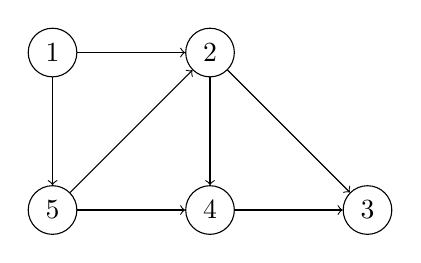
\begin{tikzpicture}
        \node[shape=circle,draw=black] (1) at (0,0) {1};
        \node[shape=circle,draw=black] (2) at (2,0) {2};
        \node[shape=circle,draw=black] (3) at (4,-2) {3};
        \node[shape=circle,draw=black] (4) at (2,-2) {4};
        \node[shape=circle,draw=black] (5) at (0,-2) {5};

        \path [->] (1) edge node[left] {} (2);
        \path [->] (2) edge node[left] {} (3);
        \path [->] (1) edge node[left] {} (5);
        \path [->] (5) edge node[left] {} (2);
        \path [->] (2) edge node[left] {} (4);
        \path [->] (5) edge node[left] {} (4);
        \path [->] (4) edge node[left] {} (3);

    \end{tikzpicture}
\end{center}

\begin{equation*}
    M = \begin{array}{c|ccccc}
    & 1 & 2 & 3 & 4 & 5 \\
    \hline
    1 & 1 & 0 & 0 & 1 & 0 \\
    2 & 0 & 0 & 1 & 1 & 0 \\
    3 & 0 & 0 & 0 & 0 & 0 \\
    4 & 0 & 1 & 0 & 0 & 0 \\
    5 & 1 & 0 & 1 & 0 & 0 \\
    \end{array}
\end{equation*}
\paragraph*{Dimensione} $|V|^2=n^2$
\paragraph*{Numero di celle con 1} $|E|$

\subsection{Esempio grafo non orientato}
\begin{center}
    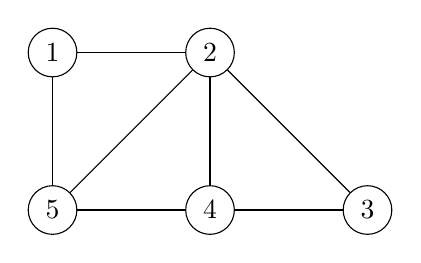
\begin{tikzpicture}
        \node[shape=circle,draw=black] (1) at (0,0) {1};
        \node[shape=circle,draw=black] (2) at (2,0) {2};
        \node[shape=circle,draw=black] (3) at (4,-2) {3};
        \node[shape=circle,draw=black] (4) at (2,-2) {4};
        \node[shape=circle,draw=black] (5) at (0,-2) {5};

        \path [-] (1) edge node[left] {} (2);
        \path [-] (2) edge node[left] {} (3);
        \path [-] (1) edge node[left] {} (5);
        \path [-] (5) edge node[left] {} (2);
        \path [-] (4) edge node[left] {} (2);
        \path [-] (5) edge node[left] {} (4);
        \path [-] (4) edge node[left] {} (3);

    \end{tikzpicture}
\end{center}

\begin{center}
    \begin{equation*}
        M = \begin{array}{c|ccccc}
          & 1 & 2 & 3 & 4 & 5 \\
        \hline
        1 & 0 & 1 & 0 & 0 & 1 \\
        2 & 1 & 0 & 1 & 1 & 1 \\
        3 & 0 & 1 & 0 & 1 & 0 \\
        4 & 0 & 1 & 1 & 0 & 1 \\
        5 & 1 & 1 & 0 & 1 & 0 \\
        \end{array}
        \end{equation*}
\end{center}
\paragraph*{Dimensione} $|V|^2=n^2$
\paragraph*{Numero di celle con 1} $2|E|$
\subsection{Liste VS Matrice (memoria)}
\paragraph*{Liste di adiacenza} Sono ottime dal punto di vista dell'occupazione dello spazio 
nel caso di Grafi sparsi con $|E|$ molto minore di $|V|^2$.
\paragraph*{Matrici di adiacenza} Risultano migliori nei grafi densi quindi quando ho
$|E|$ che si avvicina a $|V|^2$.
\subsection{Liste VS Matrice (tempo)}
\paragraph*{(u,v)} Intendiamo se i 2 vertici sono collegati.
Come tempo intendiamo il tempo per stabilire se (u,v) appartiene ad E e i tempi
sono i seguenti:
\begin{itemize}
    \item Liste di adiacenza $\rightarrow O(|E|) = O(m)$
    \item Matrice di adiacenza $\rightarrow O(1)$
\end{itemize}
\subsection{Cammino in un grafo orientato}
\paragraph*{Definizione di cammino} Sequenza $P=<v_{i_1},v_{i_2},..., v_{i_{k-1}},v_{i_k}>$
tale che $v_{i_k}$ appartiene a V per $1\leq j \leq k$ e $(v_{i_j},v_{i_{j+1}})$ appartiene
ad E per $1 \leq j < k$.
\paragraph*{Lunghezza del cammino} $k-1$ (numero di archi)
\paragraph*{Ciclo} Cammino in cui $v_{i_1}$ coincide con $v_{i_k}$
\paragraph*{Cammino semplice} Cammino in cui ogni vertice è presente una volta sola (cioè non
contiene cicli)
\paragraph*{Predecessore di $v_{i_k}$ in P} Vertice di $v_{i_{k-1}}$
\subsection{Grafo orientato pesato}
\paragraph*{Grafo} $G = (V,E,W)$
\begin{itemize}
    \item $V = \{v_1,v_2,v_3,...,v_n\}$ insieme di vertici
    \item $E= \{e_1,e_2,e_3,...,e_m\}$ insieme di archi
    \item $W:E \rightarrow R$ tale che $W(v_i,v_j) = w_{ij}$ è il peso dell'arco
    $(v_i,v_j)$
\end{itemize}
\paragraph*{Peso di un cammino} Si tratta della somma dei pesi di tutti gli
archi, formalmente: $P=<v_{i_1},v_{i_2},...,v_{i_k}> \rightarrow \sum^{k-1}_{j=1}w(v_{i_j},v_{i_{j+1}})$
\subsection{Esempio grafo orientato pesato}
\begin{center}
    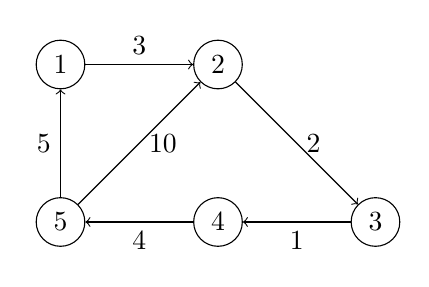
\begin{tikzpicture}
        \node[shape=circle,draw=black] (1) at (0,0) {1};
        \node[shape=circle,draw=black] (2) at (2,0) {2};
        \node[shape=circle,draw=black] (3) at (4,-2) {3};
        \node[shape=circle,draw=black] (4) at (2,-2) {4};
        \node[shape=circle,draw=black] (5) at (0,-2) {5};
    
        \path [->] (1) edge node[midway, above] {3} (2);
        \path [->] (2) edge node[midway, right] {2} (3);
        \path [->] (3) edge node[midway, below] {1} (4);
        \path [->] (4) edge node[midway, below] {4} (5);
        \path [->] (5) edge node[midway, left] {5} (1);
        \path [->] (5) edge node[midway, right] {10} (2);
        
    \end{tikzpicture}
\end{center}
\section{Il problema dei cammini minimi - Algoritmo di Floyd-Warshall}
Floyd-Warshall è un algoritmo che sfruttra la programmazione dinamica per calcolare i cammini minimi fra tutte le coppie
in un grafo orientato $G = (V,E)$. Ha un tempo di esecuzione di $\Theta(V^3)$.\\
Floyd-Warshall accetta in input grafi contenenti archi di peso negativo, ma si suppone non ci siano cicli di peso negativo.
\paragraph*{Input} Grafo $G=(V,E,W)$ (senza cappi) orientato e pesato
\paragraph*{Output} Per ogni coppia di vertici i e j, trovare il cammino di peso minimo (cammino minimo)
che parte da i e finisce in j.\\
Si tratta di un problema di ottimizzazione di minimo, dove
\begin{itemize}
    \item (n) $\rightarrow$ dimensione del problema
    \item Soluzioni possibili per una coppia di vertici i e j sono tutti i cammini da i a j
    \item Funzione obiettivo è il peso del cammino
    \item Peso del cammino minimo da i a j è il valore ottimi (per i e j)
    \item Un cammino minimo tra i vertici i e j è la soluzione ottimale
\end{itemize}
\subsection{L'input}
\paragraph*{Funzione peso W} $W:E \rightarrow R^+$ tale che $W(i,j) = w_{ij} =$ peso dell'arco $(i,j)$.
\paragraph*{Funzione peso W - Versione estesa} $W:V \times V \rightarrow R^+$ tale che $W(i,j) = w_{ij}$ con:
\begin{itemize}
    \item $w_{ij} = 0$ se $i=j$
    \item $w_{ij} =$ peso dell'arco $(i,j)$, se $(i,j) \in E$
    \item $w_{ij} = \infty$, se $i \neq j$ e $(i,j) \notin E$ 
\end{itemize}
Matrice $W=[w_{ij}]$ di n righe e n colonne.
\subsection{L'output Matrici D e $\Pi$}
\begin{itemize}
    \item Matrice $D = [d_{ij}]$ di n righe e n colonne, dove $ [d_{ij}]$ è il peso del
    cammino minimo da i e j
    \item Matrice $\Pi = [\pi_{ij}]$ di n righe e n colonne, dove $\pi_{ij}$ è il predecessore di j
    nel cammino minimo da i a j
\end{itemize}
\paragraph*{Matrice D}
\begin{itemize}
    \item $d_{ij} = 0$ se $i = j$
    \item $d_{ij} = $ peso del cammino minimo, se esiste un cammino da i a j
    \item $d_{ij} = \infty$ se non esiste un cammino da i a j
\end{itemize}
\paragraph*{Matrice $\Pi$}
\begin{itemize}
    \item $\pi_{ij} = NIL$, se $i = j$
    \item $\pi_{ij} = u$ appartenente al cammino minimo da i a j, tale che $(u,j) \in E$, se
    esiste un cammino da i a j
    \item $\pi_{ij} = NIL$, se non esisto un cammino da i a j
\end{itemize}
Dopo aver riempito entrambe le matrici mi rendo conto che:\\
\textbf{La riga i d $\Pi$ fornisce l'albero dei predecessori relativo al vertice i}.
\paragraph{Albero dei predecessori del vertice i (riga i di $\Pi$)}
\begin{itemize}
    \item $\{ j \in V | \pi_{ij} \notin NIL\} \cup \{i\} \rightarrow$ insieme dei vertici
    \item ${(\pi_{ij}, j) | \pi{ij} \notin NIL}$
\end{itemize}
\section{Sosttostruttura ottima (primo tentativo)}
Consideriamo come $P_{ij}$ il \textbf{Cammino minimo da i a j} e p è il predecessore di j.\\
Sicuramente $P_{ij} = P_{ip} + <j>$, con $P_{ip}$ cammino minimo da i a p.
\begin{center}
    \includegraphics[width=70mm, scale=0.5]{chapters_ulerich/img/floyd_warshall_tent_sottostruttura.png}
\end{center}
Con $P_{ip}$ cammino minimo da i a p. Come potrei trovare $P_{ij}$?
\begin{center}
    \includegraphics[width=70mm, scale=0.5]{chapters_ulerich/img/floyd_warshall_tent_sottostruttura_2.png}
\end{center}
\begin{enumerate}
    \item Considero tutti i vertici p' tali che $(p',j) \in E$
    \item Per ogni vertice p' determino il cammino dato da: $P_{ip} + <j>$
    \item Seleziono il cammino di peso minimo
\end{enumerate}
\paragraph*{Attenzione!} Non è sicuro che quando si calcola $P_{ij}$ si abbiano già a disposizione
i cammini $P_{ip'}$.
Si deve parametrizzare rispetto alla lunghezza I del cammino:
\begin{enumerate}
    \item Prima calcolo tutti i cammini minimi a lunghezza $0 \rightarrow P^0_{ij}$\\
    $P^0_{ij} = <i>$ se $i = j$, altrimenti $P^0_{ij} = \infty$
    \item Poi calcolo tutti i cammini minimi a lunghezza 1 $\rightarrow P^1_{ij}$\\
    $P^1_{ij} = <i,j>$ se $i \neq j$ e $(i,j) \in E$, altrimenti $P^1_{ij} = \infty$
    \item Poi calcolo tutti i cammini minimi a lunghezza 2 $\rightarrow P^2_{ij}$
    \item Poi calcolo tutti i cammini minimi a lunghezza 3 $\rightarrow P^3_{ij}$
    \item ...
    \item Ci si ferma per $l = |E| = m$ (l è lunghezza)
    \item Per ogni coppia i e j scelgo tra i cammini $P^0_{ij}, P^1_{ij}, \dots, P^m_{ij}$,
    quello di peso minimo
\end{enumerate}
\paragraph*{Friendly Reminder} $<i,j>$ Significa perorso con i vertici i e j.
\paragraph*{Domande} Come calcolo $P^l_{ij}$ con $l \geq 2$?\\
E qual è il tempo nel caso peggiore dell'algoritmo DP che sfrutta questa struttura ottima?\\
\subsection{Diamo un ordine ai vertici del grafo}
1 viene prima di 2 che viene prima di 3 etc. che viene prima dell'ultimo vertice n.\\
Parametriziamo rispetto ai vertici intermedi del cammino:
\begin{itemize}
    \item Trovo $P^0_{ij} \rightarrow$ cammino minimo senza vertici intermedi
    \item Trovo $P^1_{ij} \rightarrow$ cammino minimo con vertici intermedi $\in \{1\}$
    \item Trovo $P^2_{ij} \rightarrow$ cammino minimo con vertici intermedi $\in \{1,2\}$
    \item Trovo $P^3_{ij} \rightarrow$ cammino minimo con vertici intermedi $\in \{1,2,3\}$
    \item Trovo $P^n_{ij} \rightarrow$ cammino minimo con vertici intermedi $\in \{1,2,\dots,n\}$
\end{itemize}
\subsection*{Analizziamo nel dettaglio i cammini minimi intermedi}
$P^0_{ij} \rightarrow$ cammino minimo senza vertici intermedi.
\begin{align*}
  &P^0_{ij} = <i> \quad \text{se} \, i=j \\
  &P^0_{ij} = <i,j> \quad \text{se} \, i \neq j \text{ e } (i,j) \in E \\
  &P^0_{ij} = NIL \quad \text{se} \, i \neq j \text{ e } (i,j) \notin E
\end{align*}
Per $k > 0$, $P^k_{ij} \rightarrow$ cammino minimo con vertici intermedi $\in \{1,2,\dots,k\}$.\\
Per $k = n$, $P^n_{ij} \rightarrow$ cammino minimo con vertici intermedi $\in \{1,2,\dots,n\}$.\\
Quindi $P^n_{ij} \rightarrow$ cammino minimo $P_{ik}$.\\
\paragraph*{Sottoproblema di dimensione k} Per ogni coppia (i,j), trovare il cammino minimo
$P^k_{ij}$ dal vertice i al vertice j che ha vertici intermedi $\in \{1,2,\dots,k\}$ se $k>0$,
oppure non ha vertici intermedi se $k=0$.\\
\begin{align*}
    &k \in \{0,1,\dots,n\}\\
    &i \in \{1,\dots,n\}\\
    &j \in \{1,\dots,n\}
\end{align*}
\textbf{Numero di sottoproblemi} $n\times n \times (n+1)$.\\
$k = n \rightarrow P^n_{ij} = P_{ij}$.
\subsection{Equazioni di ricorrenza}
\paragraph*{Casi base} Sottoproblema di dimensione (0)
\begin{align*}
    &P^0_{ij} = <i> \quad \text{se } i = j\\
    &P^0_{ij} = <i, j> \quad \text{se } i \neq j \text{ e } (i,j) \in E\\
    &P^0_{ij} = NIL \quad \text{se } i \neq j \text{ e } (i,j) \notin E
\end{align*}
\paragraph*{Passo ricorsivo} Tutti i sottoproblemi di dimensione (k) tale che $k > 0$
\begin{align*}
    P^k_{ij} = ?
\end{align*}
Ricerchiamo la sottostruttura ottima.\\
\begin{center}
    \includegraphics[width=70mm, scale=0.5]{chapters_ulerich/img/floyd_warshall_tent_sottostruttura_3.png}
\end{center}
\textbf{Data una soluzione ottimale $P_{ij}=P^n_{ij}$ si possono verificare due casi:}
\begin{enumerate}
    \item Il vertice n NON è uno dei vertici intermedi
    \item Il vertice n è uno dei vertici intermedi
\end{enumerate}
\subsection*{Caso 1 - Il vertice n NON è uno dei vertici intermedi}
\begin{itemize}
    \item $P^n_{ij}$ coincide con $P^{n-1}_{ij}$
    \item Predecessore di j in $P^n_{ij}$ coincide con predecesore di j in $P^{n-1}_{ij}$
\end{itemize}
\subsection*{Caso 2 - Il vertice n è uno dei vertici intermedi}
\begin{align*}
    P^n_{ij} = P_1 + P_2
\end{align*}
\begin{center}
    \includegraphics[width=70mm, scale=0.5]{chapters_ulerich/img/floyd_warshall_tent_sottostruttura_4.png}
\end{center}
\begin{align*}
    P_1 = P^{n-1}_{in} \rightarrow P^n_{ij} = P_1 + P_2 = P^{n-1}_{in} + P_2
\end{align*}
Mentre per quanto riguarda $P_2$ avrò che
\begin{align*}
    P_2 = P^{n-1}_{nj}
\end{align*}
Quindi sostituendo $P_2$ all'interno dell'equazione avrò che:
\begin{align*}
    P_2 = P^{n-1}_{nj} \rightarrow P^n_{ij} = P_1 + P_2 = P^{n-1}_{in} + P^{n-1}_{nj}
\end{align*}
Abbiamo quindi che il predecessore di j in $P^n_{ij}$ coincide con il predecessore di j in $P^{n-1}_{nj}$.\\
\subsection*{Passo ricorsivo per $P^n_{ij}$}
La soluzione ottimale $P^n_{ij} = P_{ij}$ è data da:
\[ P^n_{ij} = min_p\{P^{n-1}_{ij}, P^{n-1}_{in} + P^{n-1}_{nj}\} \]
$i = n$ oppure $j = n \rightarrow \, P^n_{ij} = P^{n-1}_{ij}$.
\subsection*{Passo ricorsivo per $P^k_{ij}$}
La soluzione ottimale $P^k_{ij} (k>0)$ è data da:
\begin{align*}
    P^k_{ij} = min_p{P^{k-1}_{ij}, P^{k-1}{ik} + P^{k-1}_{kj}}
\end{align*}
$i=k$ oppure $j=k \rightarrow \, P^k_{ij} = P^{k-1}_{ij}$.
\subsection{Equazioni di ricorrenza}
Riassumendo abbiamo le sequenti equazioni di ricorrenza:
\paragraph*{k=0 (CASI BASE)}
\begin{align*}
    &P^0_{ij} = <i> \quad \text{se } i = j\\
    &P^0_{ij} = <i, j> \quad \text{se } i \neq j \text{ e } (i,j) \in E\\
    &P^0_{ij} = NIL \quad \text{se } i \neq j \text{ e } (i,j) \notin E
\end{align*}
\paragraph*{$k>0$ (PASSO RICORSIVO)}
\begin{align*}
    P^k_{ij} = min_p{P^{k-1}_{ij}, P^{k-1}{ik} + P^{k-1}_{kj}}
\end{align*}
\subsection*{Definizione dei coefficienti}
\textbf{Coefficienti $d^k_{ij}$ dei sottoproblemi}.\\
$d^k_{ij} \rightarrow$ peso del cammino $P^k_{ij}$
\begin{align*}
    &k \in \{0,1,\dots,n\}\\
    &i \in \{1, \dots, n\}\\
    &j \in \{1,...,n\}
\end{align*}
Quindi abbiamo \textbf{Numero di coefficienti} uguale a $n \times n \times (n+1)$.\\
$k=n \rightarrow d^n_{ij}$ è il preso $d_{ij}$ di $P_{ij}$.\\
Ricordiamo che la funzione obiettivo è trovare il peso del cammino, definiamo quindi i
coefficienti nella seguente maniera:
\paragraph*{k=0 (CASI BASE)}
\begin{align*}
    &d^0_{ij} = 0 \quad \text{se } i = j\\
    &d^0_{ij} = w_{ij} \quad \text{se } i \neq j \text{ e } (i,j) \in E\\
    &d^0_{ij} = \infty \quad \text{se } i \neq j \text{ e } (i,j) \notin E
\end{align*}
\paragraph*{$k>0$ (PASSO RICORSIVO)}
\begin{align*}
    d^k_{ij} = min_p{d^{k-1}_{ij}, d^{k-1}{ik} + d^{k-1}_{kj}}
\end{align*}
\subsection*{Predecessori $\pi^k_{ij}$}
$\pi^k_{ij} \rightarrow$ predecessore del vertice j in $P^k_{ij}$
\begin{align*}
    &k \in \{0,1,\dots,n\}\\
    &i \in \{1, \dots, n\}\\
    &j \in \{1,...,n\}
\end{align*}
\textbf{Numero di predecessori}:: $n \times n \times (n+1)$.\\
$\pi^n_{ij} \rightarrow $ predecessore $\pi_{ij}$ di j in $P_{ij}$.\\
Aggiungiamo alle equazioni di ricorrenza anche i predecessori.
\paragraph*{k=0 (CASI BASE)}
\begin{align*}
    &d^0_{ij} = 0 \quad \pi^0_{ij} = NIL \quad \text{se } i = j\\
    &d^0_{ij} = w_{ij} \quad \pi^0_{ij} = i \quad \text{se } i \neq j \text{ e } (i,j) \in E\\
    &d^0_{ij} = \infty \quad \pi^0_{ij}= NIL \quad \text{se } i \neq j \text{ e } (i,j) \notin E
\end{align*}
\paragraph*{$k>0$ (PASSO RICORSIVO)}
\begin{align*}
    &d^k_{ij} = min_p{d^{k-1}_{ij}, d^{k-1}{ik} + d^{k-1}_{kj}}\\
    &\pi^k_{ij} = \pi^{k-1}_{ij} \text{ se } d^k_{ij} = d^{k-1}_{ij} \text{ altrimenti } 
    \pi^k_{ij} = \pi^{k-1}_{kj}
\end{align*}
\section{Algoritmo bottom-up}
Per ogni valore di k da 0 a n, vengono calcolate due matrici $(n\times n)$:
\begin{align*}
    &D^k=[d^k_{ij}]\\
    &\Pi^k=[\pi^k_{ij}]
\end{align*}
Il numero totale di matrici è $2(n+1)$.
\paragraph*{Caso Base} Ho che:
\begin{align*}
    &D^0=[d^0_{ij}] = W \text{ matrice dei pesi input}\\
    &\Pi^0=[\pi^0_{ij}]
\end{align*}
\paragraph*{Passo Ricorsivo} In questo caso ho:
\begin{align*}
    &D^k=[d^k_{ij}] \text{ e } \Pi^k=[\pi^k_{ij}]\\
    &\text{ Sono calcolate usando le matrici } D^{k-1} = [d^{k-1}_{ij}] \text{ e }
    \Pi^{k-1} = [\pi^{k-1}_{ij}]
\end{align*}
Avrò quindi che le matrici $D^n = [d^n_{ij}]$ e $\Pi^n = [\pi^n_{ij}]$ sono le matrici di
output!
\subsection{Algoritmo bottom-up - Codice}
\begin{lstlisting}[language=Java, escapeinside={*@}{@*}]
    Procedura calcola_valori_ottimi_FW(V,E,W)
      *@$D^0$@* = W
      *@$\Pi^0$@* = (n x n) matrix of NIL values
      for i = 1 to n do
        for j = 1 to n do
         if i != j and *@ $w_{ij}$ != $\infty$@* then
            *@ $\Pi^0$@* [i,j] = i
      for k = 1 to n do
        for i = 1 to n do
            for j = 1 to n do
                *@$D^k[i,j] = D^{k-1}[i,j]$@*
                *@$\Pi^k[i,j] = \Pi^{k-1}[i,j]$@*
                if i != k and j != k then
                    if *@$D^k[i,j]>D^{k-1}[i,k] + D^{k-1}[k,j]$@* then
                        *@$D^k[i,j] = D^{k-1}[i,k]+ D^{k-1}[k,j]$@*
                        *@$\Pi^k[i,j] = \Pi^{k-1}[k,j]$@*
\end{lstlisting}
\paragraph*{Tempo} $\Theta(n^3)$.
\subsubsection*{Rappresentazione esecuzione algoritmo}
Link al video \href{https://www.youtube.com/watch?v=4OQeCuLYj-4&ab_channel=MichaelSambol}{Youtube}.
\chapter{Algoritmi Greedy}
Si tratta di una tecnica che si applica sempre ai problemi di ottimizzazione, ma
rispetto alla programmazione dinamica ha un approccio diverso, dato che il calcolo della
soluzione ottima (in questo caso ne calcola una sola) avviene attraverso una
sequenza di scelte \textbf{localmente} ottime.
\paragraph*{Caratteristiche degli algoritmi Greedy}
\begin{itemize}
    \item Semplici da scrivere
    \item Efficienti
\end{itemize}
\paragraph*{Questioni}
\begin{itemize}
    \item Dimostrare la correttezza di un algoritmo greedy
    \item Capire quali problemi sono affrontabili con una strategia greedy
\end{itemize}
\section{Problema - Selezione attività}
\paragraph*{INPUT} Dato un insieme $A = \{a_1, a_2, \dots, a_n\}$ di n attività, tale
che $a_i = [s_i, e_i)$ per $\ \leq i \leq n$, dove $s_i$ è il tempo di inizio ed $e_i$ è il
tempo di fine.
\begin{center}
    \includegraphics[width=80mm,scale=0.5]{greedy_sel_attivit.png}
\end{center}
$a_i=[s_i, e_i)$ e $a_j = [s_j, e_j)$ sono \textbf{compatibili} se $s_i \geq e_j$ oppure 
$s_j \geq e_i$. In poche parole se un attività inizia nello stesso momento della fine dell'altra, oppure dopo.
Le attività non devono accavallarsi, cioè eseguirsi nello stesso tempo di un'altra.
Facciamo qualche esempio che sicuramente è più semplice.\\
Per esempio $a_5=[s_5, e_5)$ e $a_8 = [s_8, e_8)$ sono compatibili, mentre $a_5 = [s_5, e_5)$ e 
$a_1 = [s_1, e_1)$ NON sono compatibili, infatti l'inizio di $a_1$ è minore della fine di $a_5$.
\paragraph*{OUTPUT} il sottoinsieme X di cardinalità massima composto di attività mutuamente compatibili.
In questo esempio l'OUTPUT desiderato è $X = \{a_2, a_5, a_7, a_8\}$.
\subsection{Soluzione con DP}
$A = \langle a_1, a_2,\dots,a_n\rangle$ tale che $e_1 \leq e_2 \leq \dots \leq e_n$.\\
$A = A \cup \{a_0, a_{n+1}\} = \langle a_0, a_1, \dots, a_n, a_{n+1}\rangle$ tale che $e_0 \leq s_1$
e $s_{n+1} \geq e_n$.
\paragraph*{Sottoproblema (i,j) per $0 \leq i < j \leq n+1$}
Trovare il sottoinsieme $X_{ij}$ di attività mutuamente compatibili di cardinalità massima per
$A_{ij} = \langle a_{i+1}, a_{i+2},\dots,a{j-2}, a{j-1} \rangle$.
\paragraph*{Sottoproblema $(0, n+1)$}
Trovare il sottoinsieme $X_{0,n+1} = X$ di attività mutuamente compatibili di cardinalità
massima per $A_{0,n+1} = \langle a_1, a_2, \dots, a_{n-1}, a_n \rangle = A$.\\
Numero totale di sottoproblemi \ra $(n+1)+n+(n-1)+(n-2)+\dots+1$.
\paragraph*{CASI BASE per $j=i+1 (A_{ij}=\emptyset)$}
$X_{ij} = \emptyset$.
\paragraph*{PASSO RICORSIVO per $j > i +1 (A_{ij} \neq \emptyset)$}
\textbf{Sottostruttura ottima}\\
$a_k$ appartiene a $X_{ij} \implies X_{ij} = X_{ik} \cup \{a_k\} \cup X_{kj}$\\
$X_{ik}$ soluzione ottima di $A_{ik}$\\
$X_{kj}$ soluzione ottima di $A_{kj}$\\
$X_{ij} = max\{X_ik \cup \{a_k\} \cup X_kj \text{ per } i < k < j\}$.
\paragraph*{Valore ottimo - Sostituzione coefficiente all'eqauzione}
\paragraph*{CASI BASE per $j=i+1 (A_{ij}=\emptyset)$}
$c_{ij} = 0$ (valore ottimo)
\paragraph*{PASSO RICORSIVO per $j > i +1 (A_{ij} \neq \emptyset)$}
$c_{ij} = max\{c_{ik} + 1 + c_kj \text{ t.c } i < k < j\}$ (valore ottimo).
\subsection{Svantaggi della Soluzione tramite DP}
\begin{enumerate}
    \item Tutti i sottoproblemi devono essere risolti per arrivare a calcolare il valore ottimo
    \item Si deve in seguito ricostruire la soluzione ottima (soluzione ottimale) perchè io ho solo
    i coefficienti, non ho la sequenza richiesta in OUTPUT
\end{enumerate}
\subsection{Approccio greedy}


\chapter{Minimum Spanning Tree - MST}
\paragraph*{INPUT}: Grafo connesso non orientato pesato $G=(V,E)$ con:\\
$W:E \rt R^+$ tale che $W(u,v)$ è il peso dell'arco (u,v).
\paragraph*{OUTPUT}: $T \subseteq E$ aciclico tale che:
\begin{enumerate}
    \item $\forall v \in V, \exists (u,v) \in T$
    \item $W(T) = \sum_{(u,v)\in T} W(u,v)$ è minimo
\end{enumerate}
$G_T = (V,T) \rt$ Minimum Spanning Tree (MST).
\begin{center}
    \includegraphics[width=80mm,scale=0.5]{minimum_spanning_tree.png}
\end{center}
$W(T)=37$
\section{Soluzione Generica}
\paragraph*{Algoritmo Generico}
\begin{enumerate}
    \item Inizializza un insieme A vuoto
    \item Aggiunge ad ogni passo un arco (u,v) in modo tale che $A \cup \{(u,v)\}$
    è sottoinsieme dell'insieme T degli archi MST
    \item L'algoritmo termina non appena $A=T$ (cioè, $G_A=(V,T)$ è MST)
\end{enumerate}
$(u,v)$ \ra arco sicuro per A (cioè appartiene a MST)
\begin{lstlisting}[language=Java, escapeinside={@*}{*@}]
    Procedura Generic_MST(G,W)
        A = @*\empt*@
        while @*$G_A = (V,A) \neq$*@ MST do
            trova arco (u,v) sicuro per A
            A = A @*$\cup$*@ {(u,v)}
        return A
\end{lstlisting}
\section{Definizioni Principali}
\subsection{Taglio}
\definizione{Definizione di Taglio: Partizione di V in due insiemi $V'$ e $V-V'$}
\subsection{Arco che Attraversa il Taglio}
\definizione{Definizione di Arco che \underline{Attraversa} il Taglio: arco $(u,v) \in E$ tale che u appartiene a $V'$ e v 
appartiene a $V'-V$} 
\paragraph*{Esempio di Taglio}
\begin{center}
    \includegraphics[width=80mm,scale=0.5]{mst_taglio.png}
\end{center}
$V' = \{1,2,3,5,6\}$\\
$V'-V=\{4,7,8,9\}$\\
\subsection{Taglio che rispetta un insieme}
\definizione{Un taglio che \underline{rispetta} un insieme $A \subseteq E$, se nessun arco di A
attraversa il taglio}
\begin{center}
    \includegraphics[width=80mm,scale=0.5]{mst_taglio_rispetta.png}
\end{center}
Il taglio rispetta $A = \{(1,2),(2,3),(3,6),(7,8),(8,9)\}$.
\subsection{Arco Leggero}
\definizione{Arco di peso minimo che attraversa il taglio}
\begin{center}
    \includegraphics[width=80mm,scale=0.5]{mst_taglio_leggero.png}
\end{center}
(4,2) \ra arco \underline{leggero}
\section{Teorema dell'arco sicuro}
Dati un grafo connesso non orientato e pesato $G=(V,E)$, un sottoinsieme A dell'insieme T di archi di un
Minimum Spanning Tree (MST) e un qualsiasi taglio che rispetti A, allora un arco leggero (u,v) del taglio è
sicuro per A, cioè $A \cup \{(u,v)\} \subseteq T$.
\subsection{Proof}
Considero T \ra insieme di archi di un MST.\\
$A \subseteq T \rt$ sottoinsieme di T.\\
Taglio che rispetta A = (\tikz \fill[green] (0,0) circle (2pt);, \tikz \fill[blue] (0,0) circle (2pt);).\\
$(u,v) \rt$ arco leggero del taglio.
\begin{center}
    \includegraphics[width=80mm,scale=0.5]{arco_sicuro_dim_mst.png}
\end{center}
Il peso $W(u,v)$ è sicuramente $\leq$ rispetto al peso $W(x,y)$.\\
Sostituisco $(x,y)$, con $(u,v)$ e inserisco quindi l'arco $(u,v)$ all'interno
del grafo e noto che il grafo resta comunque un albero, vedo che resta un MST dato
che non ci sono cicli, ottengo quindi $T'$ con $W(T') \leq W(T)$.\\
\begin{center}
    \includegraphics[width=80mm,scale=0.5]{arco_sicuro_dim_mst_2.png}
\end{center}
Per ipotesi, $A \subseteq T$ non contiene $(u,v)$ e $(x,y)$ e per costruzione $T'$ 
non contiene $(x,y)$.\\
$\implies A \subseteq T'$\\
$A \cup \{(u,v)\} \subseteq T'$
\subsection{Esempio Teorema}
Dato il seguente sottoinsieme di T denominato $A = \{archi blu\} \subseteq T$, prendiamo\\
l'arco (2,4) \ra che è arco leggero (dato che ha peso 2), posiamo dire che è un arco sicuro,
infatti se guardiamo T notiamo che $A \cup \{(2,4)\} \subseteq T$, infatti l'arco appartiene
all'MST T.
\begin{center}
    \includegraphics[width=80mm,scale=0.5]{arco_sicuro_es.png}
\end{center}
\subsection{Soluzione generica}
\begin{lstlisting}[language=Java, escapeinside={@*}{*@}]
    Procedura Generic_MST(G,W)
        A = @*\empt*@
        while @*$|V|-|A|>1$*@ do
            trova arco (u,v) sicuro per A
            A = A @*$\cup$*@ {(u,v)}
        return A
\end{lstlisting}
\begin{enumerate}
    \item A rimane aciclico durante le iterazioni
    \item $G_A = (V,A)$ (ad ogni iterazione) è una foresta di $|V|-|A|$ alberi
    \item All'inizio $G_A$ contiene $|V|$ alberti (i singoli vertici)
    \item Ogni iterazione riduce di 1 il numero di alberi e l'arco sicuro (u,v) collega
    sempre componenti distinte di $G_A$
    \item Quando si arriva a un solo albero l'algoritmo termina
    \item Il numero di iterazioni è pari a $|V|-1$
\end{enumerate}
\subsection{COROLLARIO}
$A\subseteq T$ è tale che $G_A = (V,A)$ è una foresta di $|V|-|A|$ alberi.\\
Sia $C= (V_C, A_C), V_C \subseteq V$ e $A_C \subseteq A$, una componente connessa di $G_A$\\
$\implies (V_C, V-V_C)$ è sicuramente un taglio che \underline{rispetta} A\\
$\implies$ un arco leggero di $(V_C, V-V_C)$ è arco \underline{sicuro} per A.\\
\paragraph*{QUINDI} Ad ogni iterazione, per aggiungere ad A un arco sicuro (arco di MST) basta:
\begin{enumerate}
    \item Considerare una delle componenti C della foresta $G_A = (V,A)$
    \item Trovare l'arco di peso minimo che collega un vertice in C con un vertice non in C
\end{enumerate}
\begin{center}
    \includegraphics[width=80mm,scale=0.5]{arco_sicuro_corollario.png}
\end{center}
\paragraph*{Corollario} Dati un grafo connesso non orientato e pesato G = (V,E), un
sottoinsieme A degli archi di MST, una componente connessa $C = (V_C, E_C)$ di $G_A = (V,A)$,
allora un arco leggero (u,v) del taglio $(V_C, V-V_C)$ è un arco \underline{sicuro} per A.
\subsection{Implementazione GENERIC-MST}
Ci sono principalmente due implementazioni di GENERIC-MST e sono 2 algoritmi:
\begin{itemize}
    \item Algoritmo di Kruskal
    \item Algoritmo di Prim
\end{itemize}
\section{Algoritmo di Kruskal}
\textbf{MST = Sottoinsieme ottimo di un matroide grafico $M_G$}.
$M_G = (S,F)$ per $G=(V,E,W)$ non orientato e connesso:
\begin{itemize}
    \item S, insieme E degli archi di G
    \item F, tutti i sottoinsiemi di S che sono aciclici
\end{itemize}
pesato con:\\
$W:S \rt R^+$ tale che $W(s)$ è il peso dell'arco s.\\
Sottoinsieme ottimo di $M_G$ pesato con W\\
\ra Archi dello Spanning Tree (ST) di peso massimo.\\
$W':S \rt R^+$ tale che $W'(s) = W_0 - W(s)$\\
$W_0$ è il massimo valore del peso degli archi (massimo per W)\\
Sottoinsieme ottimo di $M_G$ pesato con $W'$\\
\ra Sottoinsieme masimale di peso massimo (per $W'$) e di peso minimo per W che equivale a dire:\\
\ra Archi dello Spanning Tree (ST) di peso \underline{minimo}, cioè l'MST.
\subsection{Algoritmo Greedy Standard per il matroide grafico}.
\begin{lstlisting}[language=Java, escapeinside={@*}{*@}]
    Procedura Generic_matroid_grafic(E = @*$\{e_1, e_2, ..., e_n\}$*@)
        X = @*$\emptyset$*@
        Ordino E per peso W crescente (non decrescente)
        for i form 1 to n do
            if @*$e_i$*@ arco sicuro then
                A = @*$\{e_i\} \cup A $*@
        return A
\end{lstlisting}
\subsection{Algoritmo Kruskal}
\begin{lstlisting}[language=Java, escapeinside={@*}{*@}]
    Procedura KRUSKAL_MST(G = (V,E), W)
        A = @*$\emptyset$*@
        E = @*$\langle e_1, e_2, ..., e_n \rangle$*@ ordinati per peso crescente (non decr.)
        for i form 1 to n do
            if @*$\{e_i\} \cup A \subseteq T$*@ then
                A = @*$\{e_i\} \cup A $*@
        return A
\end{lstlisting}
Devo tradurre in codice l'if che determina se $e_i$ è un arco sicuro e per fare questo
\textbf{applico il corollario}:\\
$e_i = (u,v)$ è arco sicuro se è un arco di peso minimo che connette un vertice di una componente C
con un vertice che non è in C. Quindi $e_i$ è arco sicuro se connette due componenti diverse
di $G_A = (V,A)$. Quindi basta asssegnare l'arco che sto analizzando $e_i$ a $(u,v)$ e se
non appartengono alla stessa componente di $G_A(V,A)$, allora posso aggiungere l'arco alla soluzione A.
\begin{lstlisting}[language=Java, escapeinside={@*}{*@}]
    Procedura KRUSKAL_MST(G = (V,E), W)
        A = @*$\emptyset$*@
        E = @*$\langle e_1, e_2, ..., e_n \rangle$*@ ordinati per peso crescente (non decr.)
        for i form 1 to n do
            (u,v) = @*$e_i$*@
            if u e v @*$\notin$*@ stessa componente di @*$G_A(V,A)$*@ then
                A = @*$\{(u,v)\} \cup A $*@
        return A
\end{lstlisting}
\subsection{Esempio di Esecuzione Algoritmo Kruskal}
\paragraph*{Passo 1} Ordina E per peso non decrescente \ra $E=\langle e_1, e_2, ..., e_m\rangle$,
in modo tale da avere nell'insieme E prima gli archi più leggeri e mano a mano quelli più
pesanti, in questo modo posso applicare un approccio Greedy.\\
Inizializza $A = \emptyset$.\\
\paragraph*{Inizio a considerare gli archi} Considero $e_1 = (7,8)$, connette due componenti di
$G_A$?
\begin{center}
    \includegraphics[width=80mm, scale=0.5]{kruskal_esec1.png}
\end{center}
Sì, quindi $\implies A = \{(7,8)\}$.\\
Considero ora il secondo arco $e_2 = (2,4)$, connette due componenti di $G_A$?
\begin{center}
    \includegraphics[width=80mm,scale=0.5]{kruskal_esec2.png}
\end{center}
Sì, quindi $\implies A = \{(7,8), (2,4)\}$.\\
Saltiamo qualche passo dove aggiungiamo sempre archi perchè troviamo sempre che
gli archi considerati connettono due componenti.\\
Consideriamo l'arco $e_6=(4,6)$
\begin{center}
    \includegraphics[width=80mm,scale=0.5]{kruskal_esec3.png}
\end{center}
Notiamo che in questo caso l'arco non connette due componenti di $G_A$ (le 
componenti sono già connesse tramite altri archi, aggiungere questo arco creerebbe
un ciclo), per questo non considero questo
arco e procedo a considerare il successivo.\\
Continuo in questo modo fino a quando non ho considerato tutti gli archi. Alla fine
avrò ottenuto l'MST!
\subsection{Codice Kruskal}
Abbiamo già scritto in precedenza il codice di Kruskal, ma come possiamo tradurre le istruzioni
matematiche in codice? Riscriviamo le parti riguardante il controllo di appartenenza al grafo.
\begin{lstlisting}[language=Java, escapeinside={@*}{*@}]
    KRUSKAL-MST(G=(V,E),W)
    A = @*$\emptyset$*@
    E = @*$\langle e_1, e_2, ..., e_n \rangle$*@ ordinati per peso crescente (non decr.)
    foreach v @*$\in$*@ V do
        MAKE_SET(V)
    for 1 from 1 to n do
        (u,v) = @*$e_i$*@
        if FIND_SET(u) @*$\neq$*@ FIND_SET(v) then
            A = @*$\{(u,v)\} \cup A $*@
    return A  
\end{lstlisting}
Tramite la strutture dati FIND SET andiamo ad analizzare se aggiungendo l'arco (u,v), otteniamo
un nuovo albero (quindi connettiamo due componenti) o se abbiamo sempre lo stesso albero (quindi non stiamo
connettendo le componenti, ma stiamo generando un ciclo). se le 2 FIND SET sono diverse allora
possiamo aggiungere l'arco alla soluzione finale tramite la UNION,
altrimenti lo scarto e passo a quello successivo.
\paragraph*{Complessità Algoritmo}
\begin{itemize}
    \item L'ordinamento degli archi avrà complessità $O(|E|\log |E|)$ (Merge Sort)
    \item il MAKE SET avrà complessità $O|V|$
    \item Mentre tutto il blocco for fino a UNION ha complessità $O(|E|\alpha)$, dove
    $\alpha$ è una funzione che cresce molto lentamente che è il tempo di aggiunta degli
    elementi tramite UNION
\end{itemize}
Avendo G connesso \ra $|E| \geq |V|-1$ che possiamo approssimare a $|E|$, quindi
$(|V|+|E|\alpha)$ sarà $(2|E|\alpha)$, ma essendo il 2 un coefficiente costante nell'utilizzo
dell'O è trascurabile.\\
In totale avrò $O(|E|\log |E|+|E|\alpha)$.\\
Sicuramente $\alpha \leq \log |V|$, perchè $\alpha$ cresce molto lentamente
$|V| = |E|$, per questo motivo avrò:\\
\paragraph*{Complessità} $O(E \log|E| + |E|\log |E|)$ quindi\\
$O(|E|\log |E|)$.

\section{Algoritmo di Prim}
Altro algoritmo utilizzato per trovare l'albero di copertura minimo in un grafo che in questo
caso si basa sull'effettuare tagli e scegliere l'arco leggero (quindi sicuro).\\
Si basa sull'assegnazione di un peso ai vertici e questo è un meccanismo utilizzato anche
da un altro algoritmo che vedremo più avanti denominato Dijkstra.
\subsection{Idea dell'algoritmo}
\begin{enumerate}
    \item Sceglie un vertice arbitrario r (componente C iniziale composta dal solo
    vertice r)
    \item Trova l'arco di peso minimo che connette r a un altro vertice v
    (il vertice v entra a far parte di C)
    \item Trova l'arco di peso minimo che connette un vertice in C a un vertice
    v non in C, (il vertice v entra a far parte di C)
    \item Etc.
    \item L'algoritmo termina quando la componente C comprende tutti i vertici
    del grafo e coincide quindi con il Minimum Spanning Tree
\end{enumerate}
\subsection{Proprietà dell'algoritmo}
Ad ogni passo:
\begin{enumerate}
    \item Il sottoinsieme A degli archi di MST aggiunti, stanno tutti nella componente C.
    La foresta $G_A = (V,A)$ è composta da:
    \begin{itemize}
        \item $C = (V_C, A)$
        \item $|V-V_C|$ componenti di vertici singoli
    \end{itemize}
    \item Il taglio $(V_C, V-V_C)$ rispetta l'insieme A
    \item l'arco sicuro è l'arco di peso minimo che connette un vertice in C con
    un vertice non in C
\end{enumerate}
L'idea è quindi quella di effettuare dei tagli tali per cui $(V_C, V-V_C)$ rispetta
l'insieme A, quindi effettuo dei tagli tra l'insieme A gli archi già aggiunti
all'MST e gli altri archi e considero l'arco leggero. Per il teorema dell'arco sicuro, 
l'arco sicuro è l'arco di peso minimo che connette un vertice in C con un vertice
non i C.
\paragraph*{Esempio} Qui di seguito notiamo che effettuando il taglio e scegliendo l'arco
leggero preleviamo automaticamente l'arco sicuro.
\begin{center}
    \includegraphics[width=80mm,scale=0.5]{prim_exec1.png}
\end{center}
Continuando ad effettuare tagli validi e a selezione l'arco leggero (quindi sicuro) otteniamo
otterremo l'MST.
\subsection{Implementazione Prim}
Come possiamo implementare in maniera efficiente l'esecuzione del taglio e la
conseguente ricerca dell'arco di peso minimo?\\
Assegneremo dei pesi ai vertici e un valore contenente il suo predecessore per ogni v in V e utilizzeremo
come struttura dati una \textbf{coda Q di min-priority}.\\
La \textbf{min priority queue} è coda particolare che con l'operazione di Dequeue permette
di estrarre l'elemento di priorità minima, in questo caso ci servirà per ottenere sempre l'elemento
di peso minimo.\\
Inizializziamo i pesi a infinito e i valori del predecessore a NIL:
\begin{itemize}
    \item v.key = $\infty$
    \item v.$\pi$ = NIL
\end{itemize}
Scegliamo un \textbf{vertice r} arbitrario, che sarà il nodo d'origine dell'algoritmo. 
Nell'esempio scegliamo $r = 1$ e peso $1.key = 0$.\\
Inseriamo tutti i vertici in una coda Q di min priority che permette l'estrazione 
del vertice con il minimo valore del campo key.
\begin{center}
    \includegraphics[width=80mm,scale=0.5]{prim_impl1.png}
\end{center}
\paragraph*{Prima estrazione coda} Estraiamo ora da Q il vertice con il minimo valore di key \ra vertice 1.
\paragraph*{NB} L'estrazione implica la rimozione dell'oggetto dalla coda!\\
Procediamo quindi ad esaminare gli adiacenti di 1 \ra 2, 7, 5.\\
2 appartiene a Q and $W(1,2) < 2.key \\ \implies 2.key = (1,2);\quad 2.\pi = 1$.
\begin{center}
    \includegraphics[width=80mm,scale=0.5]{prim_impl2.png}
\end{center}
Considero il secondo adiacente, 7. Esso appartiene a Q and $W(1,7) < 7.key \\
\implies 7.key = W(1,7);\quad 7.\pi = 1$.
\begin{center}
    \includegraphics[width=80mm,scale=0.5]{prim_impl3.png}
\end{center}
Considero il terzo vertice adiacente, 5. Esso appartiene a Q and $W(1,5) < 5.key \\
\implies 5.key = W(1,5); \quad 5.\pi = 1$.
\begin{center}
    \includegraphics[width=80mm,scale=0.5]{prim_impl4.png}
\end{center}
\paragraph*{Seconda estrazione coda} Ora che ho esaurito tutti gli adiacenti procedo nuovamente a estrarre da Q il vertice
con il minimo valore di key \ra vertice 1, in questo passo si tratta del vertice 5 che ha
key = 4.\\
Esamino gli adiacenti di 5 \ra 1, 7.\\ 
1 non è più in Q, quindi lo ignoro ed esamino 7.\\
7 appartiene a Q and $W(5,7) < 7.key \\
\implies 7.key = W(5,7); \quad 7.\pi = 5$.
\paragraph*{Terza estrazione coda} Non ho più adiacenti quindi riprocedo a estrarre dalla coda Q il vertice di peso minimo,
ora si tratta del vertice 2.\\
Gli adiacenti di 2 sono 1, 4, 9, 3.\\
1 non è più nella coda, lo ignoro.\\
4 appartiene a Q and $W(2,4) < 4.key$, quindi aggiorno il suo valore di key\\
$\implies 4.key = W(2,4); \quad 4.\pi = 2$.
\paragraph*{Saltiamo qualche passaggio} Arriviamo fino al passaggio dove estraiamo
dalla coda il vertice 9. I suoi adiacenti sono 8, 2, 3, 6.\\
Questo caso è interessante perchè vediamo come effettivamente l'algoritmo trova un arco
che collega il vertice 8 di peso inferiore rispetto al precedente trovato e lo aggiorna.\\
Verifichiamo che 8 appartiene ancora a Q e inoltre $W(9,8) < 8.key$ dato che 2 $2<6\\
\implies 8.key = W(9,8);\quad 8.\pi = 9$. Viene aggiornato il predecessore con quello più
che percorre l'arco più leggero in questo momento.\\
Il vertice 2 non è più nella coda quindi non ci interessa.\\
Altro caso interessante è il vertice 3, procediamo ad analizzarlo.\\
3 appartiene a Q AND $W(9,3)$ non è $< 3.key$, perchè $14>7$, cioè sto percorrendo un arco
peggiore in termini di peso rispetto a quello percorso in precedenza, quindi non aggiorno il valore
key di 3 e lascio il suo predecessore invariato.\\
$\dots$\\
Procedo fino a quando la coda Q è vuota, in quel momento l'algoritmo termina.
\begin{center}
    \includegraphics[width=80mm,scale=0.5]{prim_impl5.png}
\end{center}
In questo momento ho esplorato tutti i vertici, ma come faccio a determinare l'MST?
\subsection{Determinare l'MST}
Considero gli archi per cui: $T = \{(v.\pi, v)\text{ t.c } v \in V, v \neq r\} \rt$ archi di MST.\\
Cioè percorro i predecessori degli archi, tranne nel caso in cui il sono nel vertice d'origine dove
$r.\pi = NIL$.\\ In questo modo ricostruisco tutto l'MST.
\subsection{Riassunto PRIM-MST}
In questo algoritmo viene mantenuta una coda Q di min-priority che all'inizio contiene tutti
i vertici del grafo e ad ogni passo Q:
\begin{itemize}
    \item contiene i vertici che non appartengono ancora alla componente C
    \item permette di estrarre il vertice v tale che (u,v) è l'arco di peso minimo che collega
    un vertice u in C con un vertice non ancora in C
\end{itemize}
Ogni vertice v del grafo ha due campi:
\begin{itemize}
    \item $v.key$ (quando v viene stratto da Q) minimo valore del peso degli archi (u,v), incidenti
    in v tali che u sia nella componente C
    \item $v.\pi$, vertice u tale che (u,v) è l'arco di peso $v.key$
\end{itemize}
All'inizio $v.key = \infty$ e $v.\pi = NIL$ per ogni vertice del grafo.\\
$r.key = 0$.
\paragraph*{Ad ogni passo}
\begin{enumerate}
    \item Viene estratto Q il vertice u con il minor valore del campo key (dato che abbiamo una
    min priority queue)
    \begin{itemize}
        \item l'arco ($u.\pi$, u) è un nuovo arco di MST
        \item u è un nuovo vertice che si aggiunge alla componente C
    \end{itemize}
    \item Per ogni vertice v adiacente a u, se v è in Q e \textbf{$v.key$} è inferiore al peso $W(u,v)$
    (ho un arco migliore del precedente), allora aggiorno i valori
    \begin{itemize}
        \item \textbf{$v.key$} al valore $W(u,v)$
        \item \textbf{$v.\pi$} al valore u
    \end{itemize}
\end{enumerate}
L'algor9itmo termina quando Q è vuota.\\
\textbf{$T = \{(v.\pi, v)\text{ t.c } v \in V, v \neq r\} \rt$  archi di MST}.
\subsection{Codice PRIM-MST}
\begin{lstlisting}[language=Java, escapeinside={@*}{*@}]
    Procedura PRIM_MST(G,W,r)
        foreach v @*$\in$*@ V do
            v.key = @*$\infty$*@
            v.@*$\pi$*@ = NIL
        r.key = 0
        Aggiungi tutti i vertici di V alla coda Q
        while Q != @*$\emptyset$*@
            u = estrai vertice da Q
            foreach v @*$\in$*@ adj(u) do
                if v @*$\in$*@ Q and W(u,v) < v.key then
                    v.key = W(u,v)
                    v.@*$\pi$*@ = u
\end{lstlisting}
\paragraph*{Complessità} La fase di inizializzazione impiega $O(|V|)$, lo stesso
per il while dato che deve scorrere tutti i vertici ($O(|V|)$). Mentre l'estrazione
richiede $O(\log |V|)$. La parte relativa agli adiacenti dipende dal numero di archi
infatti impiegherà $O(|E|)$. La parte relativa all'aggiornamento della valore key 
$O(\log |V|)$.\\
La complessità alla fine sarà di $O(|E|\log |E|)$.



\chapter{Breadth First Search - BFS}
Visita in ampiezza di un grafo non orientato
\section{Introduzione Concetti}
\subsection*{Distanza tra due vertici}
$G=(V,E) \rt$ grafo non orientato con insieme V dei vertici e insieme E degli archi.\\
\textbf{Distanza} di u da v \ra minimo numero di archi da percorrere per andare da v a u.
\paragraph*{Esempio} Distanza di 3 da 4 = 2
\begin{center}
    \includegraphics[width=80mm, scale=0.5]{bfs-esempio-pesi.png}
\end{center}
In poche parole è come se ogni arco avesse peso 1.
\subsection*{BFS(G,s) - Visita in ampiezza}
Significa effettuare la visita di un grafo \textbf{non} orientato G, a partire da un vertice
sorgente s:
\begin{itemize}
    \item All'inizio viene visitata la sorgente s
    \item Vengono poi visitati uno dopo l'altro tutti gli adiacenti di S
    \item In seguito, per ogni adiacente v di s, vengono visitati uno dopo l'altro
    gli adiacenti di v non ancora visitati
    \item Si prosegue a visitare gli adiacenti degli adiacenti e via di seguito
\end{itemize}
Tradotto in un esempio pratico:
\begin{itemize}
    \item Viene visitato s
    \item Vengono visitati tutti i vertici a distanza 1 da s
    \item Vengono visitati tutti i vertici a distanza 2 da s
    \item Vengono visitati tutti i vertici a distanza 3 da s
    \item etc.
\end{itemize}
\subsection{Caratteristiche di BFS}
\begin{itemize}
    \item Visita tutti e i soli vertici raggiungibili da s (vedremo che per DFS non sarà così)
    \item Ogni vertice del grafo viene visitato al più una volta
    \item Permette di trovare la distanza (in archi) da s di tutti i vertici
    raggiungibili dalla sorgente
\end{itemize}
\section{Colore Vertici}
I vertici hanno associato un colore:
\begin{itemize}
    \item vertice \underline{bianco} \ra vertice non visitato
    \item vertice \underline{grigio} \ra vertice visitato (adiacenti non
    completamente visitati)
    \item vertice \underline{nero} \ra vertice visitato (adiacenti completamente visitati)
\end{itemize}
\section{Esempio Esecuzione BFS}
BFS(G, A), in questo modo identifico che la sorgente è A, quindi inizio da A.
\begin{center}
    \includegraphics[width=80mm,scale=0.5]{bfs_esec1.png}
\end{center}
Controllo quali sono i nodi adiacenti ad A e $adj(A)=B,C,E$.\\
Parto da B, percorro l'arco e per segnare che ho percorso l'arco per esplorare B 
faccio diventare l'arco più spesso, inserisco B come risultato del BFS.
\begin{center}
    \includegraphics[width=80mm,scale=0.5]{bfs_esec2.png}
\end{center}
I vertici verdi indicano che la distanza dalla sorgente è 1.\\
Dopo aver visitato B, proseguo al secondo adiacente C, l'arco A-C diventa spesso 
perchè è stato percorso per scoprire C, inserisco C nella soluzione.\\
Passo ad E e faccio la stessa cosa.
\paragraph*{Coloro A di nero} Tutti gli adiacenti di A sono grigi (sono stati visitati), quindi
A diventa nero.
\paragraph*{Analizzo gli adiacenti di B}
\begin{center}
    \includegraphics[width=80mm,scale=0.5]{bfs_esec3.png}
\end{center}
Osservo che gli adiacenti sono \ra $adj(B) = D,F,C,A$.\\
Analizzo D, noto che non è stato ancora esplorato (è bianco), quindi lo coloro di grigio e
faccio diventare l'arco B-D spesso. Coloro di Giallo il vertice D per indicare distanza 2 dalla
sorgente.\\
Lo stesso per F.\\
C lo ignoro perchè è stato già esplorato in precedenza.\\
A lo ignoro perchè è nero, quindi è già completo.\\
Notiamo che gli adiacenti di B sono tutti grigi, quindi B diventa nero.
\begin{center}
    \includegraphics[width=80mm,scale=0.5]{bfs_esec4.png}
\end{center}
\paragraph*{Analizzo gli adiacenti a C} \ra $adj(C) = B,F,E,A$.\\
B lo ignoriamo perchè è nero.\\
F lo ignoriamo perchè è grigio.\\
E lo ignoriamo perchè è grigio.\\
A lo ignoriamo perchè è nero.
Tutti i vertici di C sono stati esplorati, C \ra nero.
\paragraph*{Analizzo gli adiacenti a E} \ra $adj(E) = A,C,F$.\\
A lo ignoro perchè è nero.\\
C lo ignoro perchè è nero.\\
F lo ignoro perchè è grigio.\\
Tutti i vertici di E sono stati esplorati, E \ra nero.
\paragraph*{Analizzo gli adiacenti di D} \ra $adj(D) = B, F$.\\
B lo ignoro perchè è nero.\\
F lo ignoro perchè è grigio.\\
Tutti i vertici di D sono stati esplorati, D \ra nero.
\paragraph*{Analizzo gli adiacenti a F} \ra $adj(F) = B,D,C,E$.\\
Tutti i vertici adiacenti sono neri.\\
Tutti i vertici di F sono stati esplorati, F \ra nero.
\begin{center}
    \includegraphics[width=80mm,scale=0.5]{bfs_esec5.png}
\end{center}
Questo è il risultato finale, notiamo che G e H, non sono stati esplorati, infatti sono bianchi.\\
Questo perchè BFS visita solo archi gli archi connessi alla sorgente.\\
A predecessore di B,C,E.\\
B predecessore di D,F.\\
Con questi dati otteniamo \textbf{l'Albero della BFS}:
\begin{center}
    \includegraphics[width=80mm,scale=0.4]{bfs_albero.png}
\end{center}
\section{Strutture di base della BFS}
\begin{itemize}
    \item color \ra vettore dei colori
    \item d \ra vettore delle distanze
    \item $\pi$ \ra vettore dei predecessori
\end{itemize}
\subsection*{Vettore dei colori di lunghezza $|V|$}
color[v]:
\begin{itemize}
    \item W (bianco) \ra vertice non visitato
    \item G (grigio) \ra vertice visitato (ma non tutti gli adiacenti sono già
    stati ispezionati)
    \item B (nero) \ra vertice visitato (con tutti gli adiacenti visitati)
\end{itemize}
\paragraph*{Prima e Dopo la visita}
\begin{itemize}
    \item Prima della visita \ra color[v] = W per ogni vertice v
    \item Dopo la visita \ra color[v] = W per ogni vertice v non visitato
    \item Dopo la visita \ra color[v] = B per ogni vertice v visitato
\end{itemize}
\paragraph*{Durante la visita} un vertice v che ha ancora adiacenti da ispezionare è
di colore G. Nessun vertice ha colore G prima e dopo la visita.
\subsection*{Vettore delle distanze di lunghezza $|V|$}
d[v] \ra distanza di v dalla sorgente s.
\begin{itemize}
    \item Prima delle visita \ra $d[v] = \infty$ per ogni v diverso da s.
    \item Per la sorgente \ra $d[s] = 0$.
    \item Dopo la visita \ra $d[v] = \infty$ per ogni v non visitato.
    \item Dopo la visita \ra $d[v] = n$ per ogni v visitato distante n archi da s
\end{itemize}
\subsection*{Vettore dei predecessori di lunghezza $|V|$}
$\pi[v]=u$ \ra predecessore di v nella visita (si ha $(u,v)\in E$).
\begin{itemize}
    \item prima delle visita \ra $\pi[v] = NIL$ per ogni v
    \item dopo la visita \ra $\pi[s] = NIL$
    \item dopo la visita \ra $\pi[v] = NIL$ per ogni $v (\neq s)$ non visitato
\end{itemize}
\begin{box_giallochiaro}
    {color[v] = W dopo la visita $\implies d[v] = \infty$ e $\pi[v]=NIL$}.
\end{box_giallochiaro}
\subsection{BFS utilizza una coda Q}
\begin{itemize}
    \item Un vertice viene inserito in Q non appena viene visitato
    \item Un vertive visitato rimane in Q finchè non viene estratto per esplorare
    i suoi adiacenti
    \item Quando tutti gli adiacenti di un vertie risultano visistati, il vertice
    diventa nero
    \item la visita termina quando Q è vuota
\end{itemize}
Q contiene solo i vertici grigi!
\section{Operazioni sulla coda Q}
\begin{itemize}
    \item \textbf{head(Q)} restituisce il vertice in testa
    \item \textbf{enqueue(Q, v)}, inserisce il vertice v in coda
    \item \textbf{dequeue(Q)}, elimina il vertice in testa
\end{itemize}
\section{Codice}
\begin{lstlisting}[language=Java, escapeinside={!"}{"!}]
    Procedura_BFS(G, s)
        foreach v !"$\in$"! V \ {s} do
            color[v] = W, d[v] = !"$\infty,\, \pi[v]$"! = NIL
        color[s] = G, d[s] = 0, !"$\pi$"![s] = NIL
        Q = !"$\emptyset$"!
        enqueue(Q,s)
        while Q is not !"$\emptyset$"! do
            v = head(Q)
            foreach u !"$\in$"! adj(v) do
                if color[u] is W then
                    color[u] = G
                    enqueue(Q,u)
                    d[u] = d[v]+1
                    !"$\pi$"![u] = v
            color[v] = B
            dequeue(Q)
\end{lstlisting}
\subsection{Esempio esecuzione algoritmo BFS}
Nella slide 109 di BFS è riportata l'esecuzione passo per passo dell'algoritmo con
i valori di distanza e di colore per ogni vertice, riportando la variazione
passo per passo.\\
Risulta ancora più evidente che la coda contiene solo vertici grigi, dato che vengono inseriti
quando vengono scoperti e rimossi solo quando diventano neri.\\
La differenza con l'esecuzione grafica è che qua chiaramente al posto dei colori ci saranno le distanze
salvate nelle tabelle e il predecessore, quindi quando scopro un nuovo vertice
devo incrementare la distanza di 1 e aggiungere il vertice che sto analizzando 
(quello prelevato dalla coda tramite la head) come predecessore del vertice adiacente che
sto considerando (quello dentro il foreach).\\
Vediamo che grazie alla coda riusciamo a mantenere in memoria tutti i vertici grigi
e mano a mano che finiamo di analizzare i vertici effettuiamo la dequeue, quindi
quando la coda sarà vuota l'algoritmo termina.
\paragraph*{Alla fine dell'esecuzione avremo la seguente tabella}
\begin{center}
    \includegraphics[width=80mm,scale=0.5]{bfs_tabella.png}
\end{center}
Per calcolare il il BFS Tree è sufficiente guardare quali sono i predecessori nella tabella,
questi sono i collegamenti che determinano l'albero di esplorazione BFS.
\subsection{BFS Tree}
$T = (V_T, E_T)$:
\begin{itemize}
    \item $V_T = \{v \in V | color[v] = B\}$
    \item $E_T = \{(\pi[v], v) | v \in V_T\}$
\end{itemize}
\subsection{Complessità in tempo}
$|V| \rt$ numero dei vertici del grafo.\\
$|E| \rt$ numero archi ndel grafo.--redirect-gateway def1
\begin{itemize}
    \item Costo di inizializzazione \ra $O(|V|)$
    \item Singola operazione su Q \ra tempo costante
    \item un vertice viene aggiunto a Q al più una volta
    \item un vertice viene estratto da Q al più una volta
    \item Ogni lista di adiacenza viene ispezionata quado il vertice viene estratto da Q
    (al più una volta)
    \item Dimebnsione totale delle liste di adiacenza \ra $2|E|$
    \item Costo di ispezioni delle liste di adiacenza \ra $O(|E|)$
\end{itemize}
\paragraph*{Complessità nel caso peggiore} $O(|V|+|E|)$
\section{Esercizi}
Sono stati proposti una serie di esercizi che richiedono l'utlizzo di BFS, per
esempio:
\paragraph*{Verificare se un grafo G=(V,E) è connesso}
\begin{lstlisting}[language=Java, escapeinside={!"}{"!}]
    Procedura Is_connected(G)
        u = randm vertex from V
        BFS(G,u)
        foreach v !"$\in$"! V do
            if colour[v] is W then
                return false
        return true
\end{lstlisting}

\chapter{Depth First Search (DFS)}

\end{document}